\documentclass[twoside,11pt]{article}
\usepackage{jmlr2e}
\usepackage{graphicx}
\graphicspath{ {./images/} }
\usepackage{enumitem}
\newlist{mylistenv}{enumerate}{3}
\newenvironment{mylist}[1]{%
	\setlist[mylistenv]{label=#1\arabic{mylistenvi}.,ref=#1\arabic{mylistenvi}}%
	\setlist[mylistenv,2]{label=#1\arabic{mylistenvi}.\arabic{mylistenvii}.,ref=#1\arabic{mylistenvi}.\arabic{mylistenvii}}%
	\setlist[mylistenv,3]{label=#1\arabic{mylistenvi}.\arabic{mylistenvii}.\arabic{mylistenviii}.,ref=#1\arabic{mylistenvi}.\arabic{mylistenvii}.\arabic{mylistenviii}}%
	\renewenvironment{mylist}{\begin{mylistenv}}{\end{mylistenv}}
	\begin{mylistenv}%
	}{%
	\end{mylistenv}%
}
\newcommand\tab[1][1cm]{\hspace*{#1}}

% Definitions of handy macros can go here

\newcommand{\dataset}{{\cal D}}
\newcommand{\fracpartial}[2]{\frac{\partial #1}{\partial  #2}}


\firstpageno{1}

\begin{document}

\title{Project 2: \textit{k} Nearest Neighbors}

\author{\name Sarah Wilson 
	   \email swi1s117@jhu.edu \\
	   \phone 303-921-7225 \\
       \addr Engineering Professionals Computer Science\\
       Johns Hopkins University\\
       Baltimore, MD 21218, USA} 

\maketitle


\section{Introduction}
Regression and classification are both common tasks in the realm of Machine Learning. Regression and classification are both supervised learning problems. Supervised learning is where the system is given an input and output and then asked to learn or predict the mapping of input to output. The algorithm explored in this paper is \textit{K}-Nearest Neighbor (\textit{K}NN). \textit{K}NN is an example of a nonparametric algorithm, nonparametic algorithms do not make any strong assumptions about the form of the mapping function from input data to output predictions. The advantage offered by this approach is that not a lot of prior knowledge on the data or its features is required to build a predictor. \textit{K}NN is nonparametric as it makes predictions for new data based upon training data by looking at the \textit{k} closest neighbors to the new data. The primary philosophy behind the \textit{k}NN algorithm is "In nonparametric estimation, all we assume is that similar inputs have similar outputs. This is a reasonable assumption: the world is smooth, and functions, whether they are densities, discriminants, or regression functions change slowly. Similar instances mean similar things. We all love our neighbors because they are so much like us."(1. Alpaydin)\\ 

\hspace*{10mm} The problem statement presented in this paper is to understand and implement a \textit{k}NN classifier and regressor on 6 different and unique data sets. The experimentation will first be tuned using a validation subset of the overall data set under experimentation, to determine the most optimal value of \textit{k} to use. Then the optimal value of \textit{k} will be run through the full \textit{k}-fold cross validation process. The experimentation will examine: \textit{k}NN, edited \textit{k}NN and condensed \textit{k}NN The results presented will be the classification error and the regression mean squared error on each of the 6 unique data sets and across the 3 variations of the  \textit{k}NN algorithm.\\

\hspace*{10mm} The hypothesis of this report is that for the Classification tasks, normal KNN will do better at classifying an instance when compared with Edited or Condensed KNN. For Regression tasks it is hypothesized, that Edited or Condensed KNN will be better at regressing a new instance than normal KNN and that results from Edited and Condensed will be reality similar. This hypothesis will be tested by looking at 6 unique data sets, 3 of which that are classification task, 3 of which that are regression tasks. These data sets will be optimally tuned for the value of K nearest neighbors to use, the $\sigma$ value to use in the Gaussian Kernel for regression, and the $\epsilon$ to use when running Condensed or Edited KNN. The results of these experiments will be discussed and presented against the outlined hypothesis. \\

\hspace*{10mm} Section 1 has provided the introduction, problem statement and hypothesis in regards to the \textit{k}NN algorithm. Section 2 will provide an in-depth explanation of the \textit{k}NN algorithm, how the algorithm will be tuned and specifics on each of the 6 data sets used. Section 3 will present the results obtained by variations of \textit{k}NN, edited \textit{k}NN and condensed \textit{k}NN and the values that were chosen as part of the tuning process. Section 4 will discuss the results that were obtained and compare them to the hypothesis that was outlined in the introduction. This report will conclude in Section 5 with a discussion of lessons learned and areas of possible future work.\newline



\section{Algorithms and Experimental Methods}
The experimental method used in this report is \textit{k}-Fold Cross Validation. \textit{k}-Fold Cross Validation is used when the data sets that an algorithm is being experimented on is small, the goal of \textit{k}-Fold Cross validation is to maximize the amount of data that is used for training of the algorithm. The experiment will use 5-Fold Cross Validation ($\textit{k} = 5$).\\ 
For the experiment in this report a Validation / Tuning set is first used to determine the optimal value of \textit{k} neighbors in the \textit{k}NN, $\sigma$ in the case of regression and $\epsilon$ in the case of Condensed or Edited KNN. \\ 

\noindent \textbf{General \textit{k}NN}\newline
For General KNN the Entire Data set is loaded, and randomly shuffled.\newline
The validation and tune process is started by removing 20\% of the observations from Entire data set, and assigning them to new Validation / Tune  data set.\newline
A list of k nearest neighbors is assigned, and the 5 fold cross validation process will be run on each value of k to determine the optimal k. In regression the Gaussian Kernel is also applied so the bandwidth of that kernel $\sigma$ is also optimized during this time. (Consider k and $\sigma$ to running in a nested for loop during the tuning process.) For classification there is no $\sigma$, so only k needs to be tuned.\newline 
The Validation / Tune Data set is broken into 5 folds. 1 of those folds is assigned as the Test fold, while the other folds are concatenated together to form the Train folds. The fold that is assigned as the test fold rotates through all 5 fold positions.\newline
For each observation in the Test Set, the distance is calculated to each observation in the Train Set using the euclidean Distance Equation. 
 $d\left( p,q\right)   = \sqrt {\sum _{i=1}^{n}  \left( q_{i}-p_{i}\right)^2 } $\newline
Where $p$ is the observation in the test set or the Query Point, and $q$ is the observation in the train set. These values are also vectors, so the full form of this equation is scaled to the number of attributes that are in each data set. 
The predictor attribute in each of the data sets is dropped from this distance calculation, as we only want to use attributes that determine the predictor, not the predictor itself.\newline
Sort the distances in an overall list for the Query Point sorted from smallest to largest.\newline
Take the K defined smallest values from that list\newline 
If running Classification return the most commonly occurring predictor value based on those K nearest neighbors.\newline 
If running regression, take these K nearest distance values and apply the Gaussian Kernel based on the $\sigma$ that we are running. The Gaussian Kernel is described by the equation: 
$\exp {\frac{-1}{2\sigma} * d\left( p,q\right)}$\newline
Each of the K nearest distances values has this Kernel applied. This Kernel is then used to determine the weighted average to come up with Regression prediction value. What specifically is meant by that is that each closest predictor value is then multiplied by its corresponding Gaussian Kernel value and then each one is summed, and divided by the sum of the Gaussian Kernel distances. 
This can be expressed as:\newline
$Weighted Prediction = \frac{(Predictor1*GK(dist1) + Predictor2*GK(dist2))...PredictorK*GK(distK)}{GK(dist1) + GK(dist2)....GK(distK)}$\newline
\newline
Where $K$ represents up to the Kth nearest neighbor. This weighted average provides a predicted value, this predicted value is then compared to the actual predicted value as determined by the Test Set or Query point. The error reported between the predicted and actual value is the Root Mean Squared Error. Root Mean Squared Error was used, since it provides how far off a measurement was in the units of the measurement that was taken. The higher the Root Mean Squared Error, the worse the prediction was to the actual value. Low Root Mean Squared Error is the objective.\newline
Once every observation in the Test Set is Compared to the Train Set, the Fold is completed. 
This process then repeats for all 5 folds. The Classification Error and Regression (RMSE) are then used to determine what the optimal values of K and $\sigma$ are to run the full experiment.\newline

The full experiment for Normal KNN is completed using the optimized K and $\sigma$, and on the other 80\% of the data that was not used as part of tuning. The process is exactly the same as what was outlined for tuning, with instead an optimized K and $\sigma$. And again the 5 Fold Cross Validation is performed.\newline 


\textbf{Edited \textit{k}NN}\\
\hspace*{10mm} Edited KNN follows the same steps that were outlined above in regards to the 5 fold cross validation, classification and application of the Gaussian Kernel for regression. The major difference is in the generation of the Training set. Instead of just taking the Training Set as it is, first we edit out the outliers from the Training Set based on their distance from the K nearest data points. 
When the Training Set is created, we loop over every observation INSIDE the training set, not the test set, essentially the Query Point has changed. The process then still remains the same, the distance to all other observations in the Train Set is calculated with respect to the Query Inside the Test set.\newline 
If the task is Classification, we get the closest K neighbors, determine the majority predictor value. If the Train Set Query point does not mach the majority predictor, then it is dropped completely from the data set. This dropping is the editing. 
If the task is Regression, we get the closest K neighbors, determine the predictor based on the application of the Gaussian Kernel / Weighted Average. We define an $\epsilon$, this $\epsilon$ is then used in the equation $|Current Query Predictor - Weighted Average Prediction| \leq \epsilon$.\newline
If the delta between the Current observation in the Train Set and the Weighted Average provided by the K nearest neighbors, is less than $\epsilon$, this data point is dropped from the Train Set.\newline

Once the values have been dropped from the Train Set, then the Normal KNN Classification / Regression process takes place. (Here the Query Point is derived from the Test Set, and we run against our Edited Train Set and all other Error parameters are reported exactly as described in the Normal KNN description.)\newline

$\epsilon$ is tuned for using 20\% of the entire data set that was set aside for validation. Once an optimal $\epsilon$ is determined then the full experiment is run using the other 80\% of the data.\newline

\textbf{Condensed \textit{k}NN}\\
\hspace*{10mm} Edited KNN follows the same steps that were outlined above in regards to the 5 fold cross validation, classification and application of the Gaussian Kernel for regression. The major difference is in the generation of the Training set, much liked Edited KNN. In the case of Condensed nearest neighbors, the Training Set is built. Each observation point in the Training Set is examined, if running classification we get the closest K neighbors to the Query from the Training Set, determine the majority predictor value. If the Train Set Query point does mach the majority predictor, then it is added to the Condensed Training Set from the data set. The addition of these observations is what makes this condensed KNN. If the task is Regression, we get the closest K neighbors, determine the predictor based on the application of the Gaussian Kernel / Weighted Average. We define an $\epsilon$, this $\epsilon$ is then used in the equation $|Current Query Predictor - Weighted Average Prediction| \leq \epsilon$.\newline
If the delta between the Current observation in the Train Set and the Weighted Average provided by the K nearest neighbors, is less than epsilon this data point is added to the newly formed Condensed Train Set.\newline

Once the values have been added from the Train Set, then the Normal KNN Classification / Regression process takes place. (Here the Query Point is derived from the Test Set, and we run against our Edited Train Set and all other Error parameters are reported exactly as described in the Normal KNN description.)\newline

$\epsilon$ is tuned for using 20\% of the entire data set that was set aside for validation. Once an optimal $\epsilon$ is determined then the full experiment is run using the other 80\% of the data.

\newpage
{\noindent}{\bf Data Sets}\newline
The following data sets were used during the classification and regression tasks for this project.\newline
{\bf Breast Cancer}\newline
Description: \newline
Task: Classification\newline
Predictor: Diagnosis (Malignant or Benign)\newline
Link:\newline \url{https://archive.ics.uci.edu/ml/datasets/Breast+Cancer+Wisconsin+%28Original%29}\newline
{\noindent}\textbf{Car Evaluation}\newline
Description:\newline
Task: Classification\newline
Predictor: Car Evaluation (Unacceptable, Acceptable, Good, Very Good)\newline
Link: \newline
\url{https://archive.ics.uci.edu/ml/datasets/Car+Evaluation}\\
{\noindent}\textbf{Congressional Vote}\newline
Description: 1984 United Stated Congressional Voting Records\newline
Task: Classification \newline
Predictor: Party (Republican / Democrat) \newline
Link: \newline
\url{https://archive.ics.uci.edu/ml/datasets/Congressional+Voting+Records}\newline
{\noindent}\textbf{Albalone}\newline
Description: Physical measurements of Albalone\newline
Task: Regression\newline
Predictor: Rings (int)\newline
Link: \newline
\url{https://archive.ics.uci.edu/ml/datasets/Abalone}\newline
{\noindent}\textbf{Computer Hardware}\newline
Description: Relative CPU performance data.\newline
Task: Regression\newline
Predictor: PRP\newline
Link: \newline
\url{https://archive.ics.uci.edu/ml/datasets/Computer+Hardware}\newline
{\noindent}\textbf{Forest Fires}\newline
Description: Forest Fire burn area data\newline
Task: Regression\newline
Predictor: Area (float)\newline
Link: \newline
\url{https://archive.ics.uci.edu/ml/datasets/Forest+Fires}\newline
	
\newpage

\section{Results}
Tables 1-9 display the results from Classification Tasks: the Breast Cancer, Car Evaluation and Congressional Vote data sets while running Normal KNN, Edited KNN and Condensed KNN. These tables show the results from the train set and the test set during each fold of the \textit{k}-fold validation process. The results of the tuning process were omitted from this report for brevity but can be found in the project submission, under Results Output. Each KNN variation was run using the optimal values as determined by the parameter tuning. Discussion of the tuning process will occur in the discussion section. The error used is classification error and can be described as the Number of Times Prediction was Wrong / Total Number of Comparisons. This error was averaged across the 5 folds to provide the Average Classification Error against each data set.\\
Tables 10-18 display the results from the Regression Tasks: the Albalone, Computer Hardware and Forest Fire data sets. These tables show the result from the train set and the test set during each fold of the \textit{k}-fold validation process.The results of the tuning process were omitted from this report for brevity but can be found in the project submission, under Results Output. Each KNN variation was run using the optimal values as determined by the parameter tuning. Discussion of the tuning process will occur in the discussion section. The error used is Root Mean Square Error. Root Mean Squared Error was used, since it provides how far off a measurement was in the units of the measurement that was taken. The higher the Root Mean Squared Error, the worse the prediction was to the actual value. Low Root Mean Squared Error is the objective.\newline

\begin{table}[h]
		\centering
		\caption{Car Evaluation: KNN - Experimental Results}
		\label{tab:table1}
		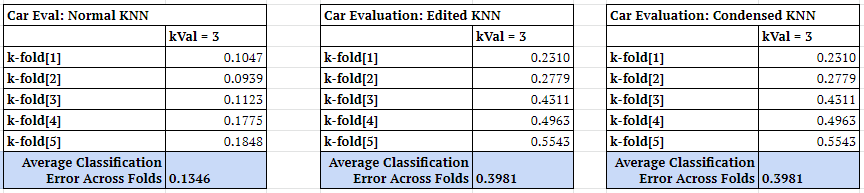
\includegraphics[scale=.7]{CV_ALL_Results}\newline
\end{table}

\begin{table}[h]
		\centering
		\caption{Breast Cancer: KNN - Experimental Results}
		\label{tab:table2}
		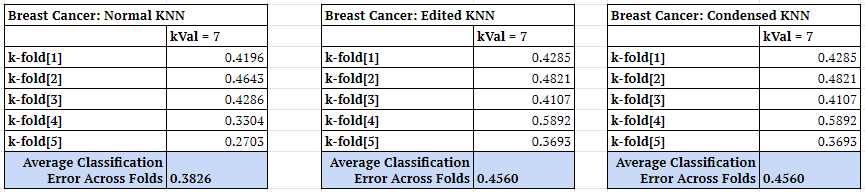
\includegraphics[scale=.7]{BC_ALL_Results}\newline
\end{table}

\begin{table}[h]
		\centering
		\caption{Congressional Vote: KNN - Experimental Results}
		\label{tab:table3}
		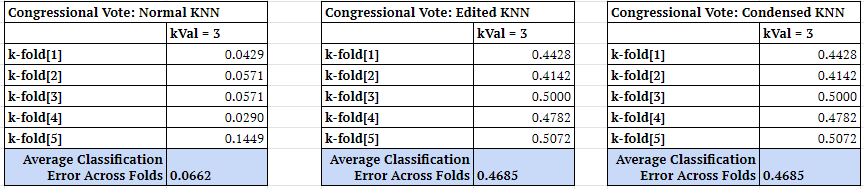
\includegraphics[scale=.7]{CVote_ALL_Results}\newline
\end{table}

\begin{table}[h]
	\centering
	\caption{Albalone: KNN - Experimental Results}
	\label{tab:table4}
	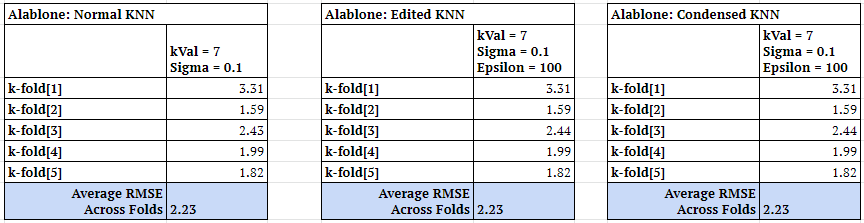
\includegraphics[scale=.7]{ABL_ALL_Results}\newline
\end{table}

\begin{table}[h]
	\centering
	\caption{Computer Hardware: KNN - Experimental Results}
	\label{tab:tale5}
	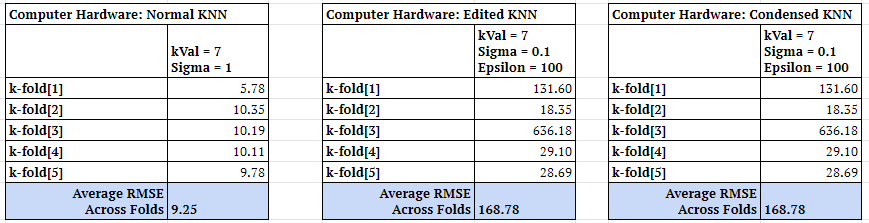
\includegraphics[scale=.7]{CH_ALL_Results}\newline
\end{table}

\begin{table}[h]
	\centering
	\caption{Forest Fires: KNN - Experimental Results}
	\label{tab:table6}
	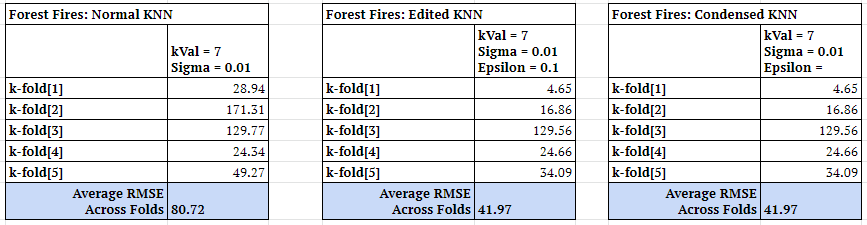
\includegraphics[scale=.7]{FF_ALL_Results}\newline
\end{table}





\newpage
\newline
\section{Discussion}
\hspace*{10mm} The hypothesis presented at the start of this report was that for the Classification tasks, normal KNN will do better at classifying an instance when compared with Edited or Condensed KNN. For Regression tasks it is hypothesized, that Edited or Condensed KNN will be better at regressing a new instance than normal KNN and that results from Edited and Condensed will be reality similar.\\
\hspace*{10mm} Looking at Classification results from the Congressional Vote, Breast Cancer and Car Evaluation data sets, it can be seen that the average classification error across the 5 folds, is lower than when compared with the average classification error from the edited and condensed experiments. These results seem to support the hypothesis. It may also be possible to see that based on the implementation details of the condensed and edited KNN, for classification a query is removed from the train set based solely on if it matches the classification of it's neighbors. If one predictor was dominate in train set compared to other, then outliers would get toss quickly. This same adding / removal process is not applied to the test set. Meaning that outliers that are naturally occurring in the Test Set, will be counted against the correct prediction count, leading to higher error. It can be noted that looking across all three data sets, the Edited KNN and Condensed KNN when looking at a specific data set are exactly equal. This seems suspect. It can be suspected that this is an error in the implementation code with the shuffling. The Entire Data Sets were not being shuffled prior to insertion into the KNN algorithm. If the random shuffling was occurring it would be likely that the results obtained for Edited and Condensed KNN in a data set would be similar, but not identical.\\
\hspace*{10mm} Looking at the Regression results from the Computer Hardware, Alablone and Forest Fire data sets, in all three cases the RMSE values obtained from the Edited and Condensed are lower than the values obtained for Normal KNN. For regression, based on implementation this would seem to make sense, you're defining a range $\epsilon$ that predictions are allowed to match to in order to be added or removed as outliers or inliers. This tuning seems to be less susceptible to the fault identified for classification, since you're defined a range of values $\epsilon$ that can be let into the Train Set, there are more chances to not over edit the data. Again the Condensed and Edited results were exactly the same, this is most likely due to the shuffling error identified as par of classification. This is my best guess assumption as to what may be happening there, a full root cause investigation would need to be had in order to determine if that is true. 

\section{Conclusion}
\hspace*{10mm} The problem statement presented in this paper is to understand and implement a \textit{k}NN classifier and regressor on 6 different and unique data sets. That objective was met, through the explanation provided in Section 2 on the different variations of KNN, normal KNN, edited KNN and condensed KNN. During the implementation, tuning and review of the results, a few areas of improvement could have been applied. The results obtained from the Edited and Condensed nearest neighbors was the same inside compared unique data sets, the root cause for this discrepancy is most likely caused by and error in the implementation code where the Entire Data Sets were not being shuffled prior to insertion into the KNN algorithm. If the random shuffling was occurring it would be likely that the results obtained for Edited and Condensed KNN in a data set would be similar, but not identical. During the course of this project, tuning was introduced and it appears that different values of k, $\sigma$, and $\epsilon$ do impact the accuracy of the results that are seen out of the prediction algorithms. An area of future work would be to explore the different types of distance calculations that could be applied to the K Nearest Neighbors problem, such as Hamming or Manhattan, and seeing if one is better suited to a particular type of Learning problem.  

\section{References}
1. Alpaydin, E. (2004). Introduction to machine learning (Oip). Mit Press. 

\newpage


\end{document}